\section{Introduction}\label{sec:intro}

The goal of the OpenDreamKit project \cite{ODKproposal:on} is to develop a generic Toolkit
that will enable Mathematicians (and scientists in general) to build so-called Virtual
Research Environments (VREs) that are optimally tailored to specific communities. These
will combine a multitude of different tasks, such as symbolic mathematics, automatic code
generation, numerical computation, data bases, post-processing or visualisation. A VRE
will provide end-users with a single tool-chain that can be used for most, if not all, of
their research.

To be able to build such a toolkit, we will need to combine three different aspects of
``doing mathematics research'' -- Data (D), Knowledge (K) and Software (S). Ultimately we want to
create and make use of them using a VRE; we want to model the real world, translate it
into a set of mathematical objects and computationally simulate and thereby explore them.

The \emph{Data Aspect} is commonly implemented in special databases as tables or lists of
numerical of symbolic data. The \emph{Systems Aspect} is represented by mathematical
software systems, such as \GAP, \SageMath, and others computing on top of this data. The
\emph{Knowledge Aspect} specifies the meaning of the mathematics data as well as the
knowledge underlying the algorithms and thus bridges between the former two. An
illustration with more examples of these aspects can be found in
Figure~\ref{fig:thebigpicture} (from the \pn proposal).

\begin{figure}[ht]\centering
  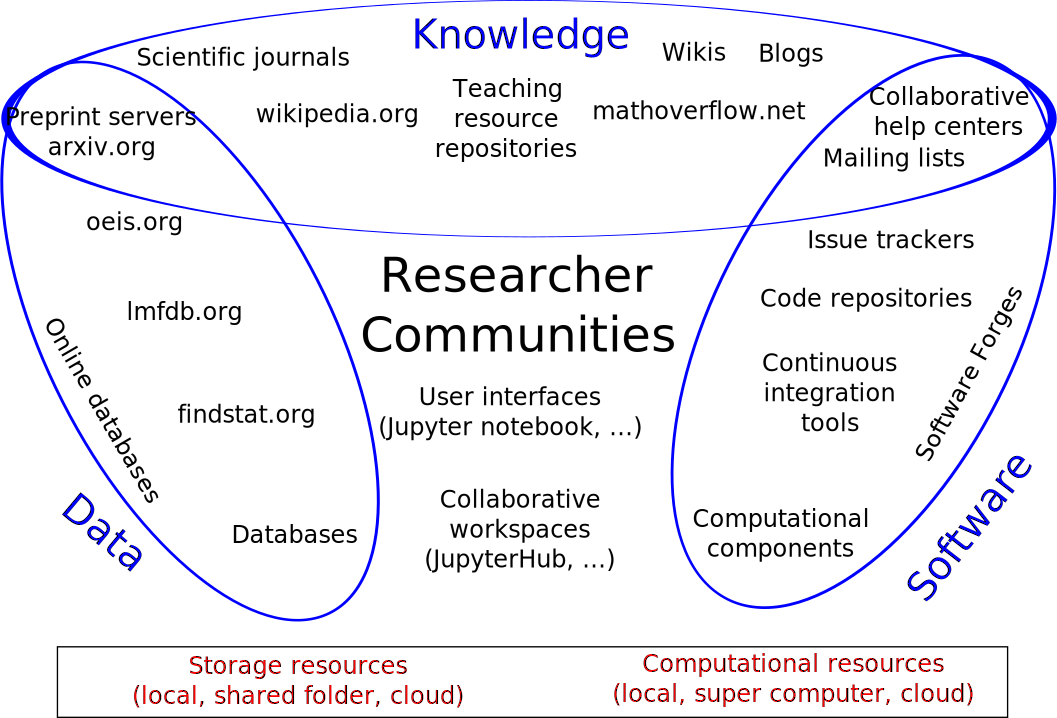
\includegraphics[width=\textwidth]{../../Proposal/Pictures/TheBigPicture.pdf}
  \caption{Virtual Research Environments for research in pure
    mathematics and applications.}
  \label{fig:thebigpicture}
\end{figure}

The approach of work package \WPtref{dksbases} in the \pn project is to model all three
aspects of mathematics research explicitly in as a basis for the envisioned mathematical
VRE toolkit. Concretely, the \pn proposal calls for an extension of the well-established
framework of theory graphs -- developed for the representation of mathematical knowledge
and languages (see Section~\ref{sec:MMT}) -- with Data and Software components to arrive
at a foundation for mathematical $\mathcal{DKS}$-bases. This deliverable report surveys
the results of the first year and presents the initial design for the
$\mathcal{DKS}$-bases.

In a series of workshops (September 2015 in Paris, January 2016 in St. Andrews, June 2016
in Bremen, and July 2016 in Bia{\l}ystok) the participants working on \WPref{dksbases} met
and discussed the topic of integrating the \pn systems into a mathematical VRE toolkit by
explicitly representing the D/K/S aspects of mathematical research and basing
computational services and inter-system communication on a joint $\mathcal{DKS}$-base. The
group agreed that for the \emph{Software Aspect}, interoperability of systems is most
important for \pn and can be achieved by aligning the mathematical knowledge underlying
the systems; this realization is engrained in the ``Math-in-the-Middle'' (MitM)
paradigm~\cite{DehKohKon:iop16}, see Section~\ref{sec:mitm} for the \emph{Software Aspect}
in \pn.

In the rest of the introduction we will 
\begin{compactenum}
\item introduce the framework of OMDoc/MMT theory graphs (Section~\ref{sec:MMT}) as a
  basis towards building DKS theories we use the \MMT system -- our existing
  implementation of theory graphs -- which has K(nowledge) theories already 
\item review the MitM paradigm for integrating the \emph{software} and \emph{knowledge}
  aspects in \pn, and
\item preview the initial design of $\mathcal{DKS}$-Bases.
\end{compactenum}
In Section~\ref{sec:survey} we report on the initial survey of existing \pn-systems with
D/K/S aspects (see also Appendix~\ref{sec:raw-survey}) conducted at the Paris workshop in
September 2015 and derive requirements from that.  Section~\ref{sec:data} introduces the
(abstract) concept of DK-theories that extend of OMDoc/MMT theory graphs for handling data
and Section~\ref{sec:impl} presents first steps towards an implementation in the MMT
system, which are then evaluated on two case studies of mathematical data bases in
Section~\ref{sec:cases}. In Section~\ref{sec:querying} how we plan to enable users to
query and make further use of DK-theories before finally concluding with a short summary
and outlook in Section~\ref{sec:conclusion}.

\subsection{A Brief Recap of Theory Graphs}\label{sec:MMT}

An OMDoc/MMT theory graph consists of theories and the relations between
them~\cite{RabKoh:WSMSML13}. An OMDoc/MMT theory is a set of declarations -- a set of
declared symbols. In addition to the declarations, each theory has a name (which together
with its namespace forms the global URI for the theory) and a meta-theory. A meta-theory
is commonly the logical framework that is used to model the content of the theory. Each
declared symbol has a name and can additionally have a type, a definition and different
kinds of meta-data. In each theory these symbols can then be used to form terms that can
be used to express more advanced knowledge. Here terms are effectively OpenMath 2.0
\cite{BusCapCar:2oms04} objects -- they mostly consist of literal values, symbols and
applications of terms to other terms.

There are two basic kinds of relations between theories: imports and views. An import is a
way to declare symbols from one theory in another theory -- to import the symbols from a
source theory to a target theory. This can for example be used to extend an existing
theory without re-declaring all symbols or to combine two theories. Furthermore the
concept of imports allows to modularise knowledge. On top of imports there are also
Structures which are imports and additional renamings of the imported symbols. The second
type of relation, the view, is a mapping from one theory to another -- a way to ``view''
one theory as another. This mapping allows terms from one theory to be translated into
another theory. In the case where terms represent boolean statements or proofs, the
mapping given by the view is truth preserving -- \emph{i.e.}~if a statement is true in the
source theory, it is be true in the target theory after translation.

Theory graphs are implemented inside the \MMT system~\cite{Rabe:MAGMS13,uniformal:on}. The
system allows for the declaration of theories along with symbols, imports and
views. Furthermore it is possible to create terms over these theories and translate them
along views. The \MMT system also provides a type checker that can be used to type check
declarations.

\subsection{Using the Math-In-The-Middle approach to integrate systems}\label{sec:mitm}

When integrating multiple systems we are mostly talking about using concrete algorithms
(implemented by these systems) to solve specific computational problems (the knowledge
about the problem). To integrate multiple systems with this knowledge we want to enable
users to write down a problem in one system and then solve it in another system. We want
to be independent of the implementation of the knowledge -- independent of the systems.

For this we make use of an approach we call ``Math-In-The-Middle'' paradigm
(see~\cite{DehKohKon:iop16} for details). Here the underlying mathematical knowledge, the
``real math'', is used as a reference ontology for system (in the ``middle'') -- hence the
name. Each system needs access to this knowledge. As each of them come with their own
particularities, they will need some interface to it.

We want to make use of the modular approach to mathematics provided by theory graphs, and
in particular \MMT as an implementation thereof, to first of all allow us translate
mathematical expressions between systems. We define a ``Math In The Middle'' theory as
well as interface theories for each system. With the help of \MMT and bi-views\footnote{A
  bi-view is a bidirectional view between two theories} between the interface theories and
the central theory, we can translate objects from one system to the other.

\begin{figure}[ht]\centering
  \def\myxscale{3}\def\myyscale{1.2}
  \documentclass{standalone}
\usepackage[mh]{mikoslides}
% this file defines root path local repository
\defpath{MathHub}{/Users/kohlhase/localmh/MathHub}
\mhcurrentrepos{MiKoMH/talks}
\libinput{WApersons}
% we also set the base URI for the LaTeXML transformation
\baseURI[\MathHub{}]{https://mathhub.info/MiKoMH/talks}

\usetikzlibrary{backgrounds,shapes,fit,shadows,mmt}
\begin{document}
\begin{tikzpicture}[xscale=2.4,yscale=.9]
  \tikzstyle{withshadow}=[draw,drop shadow={opacity=.5},fill=white]
   \tikzstyle{database} = [cylinder,cylinder uses custom fill,
      cylinder body fill=yellow!50,cylinder end fill=yellow!50,
      shape border rotate=90,
      aspect=0.25,draw]
   \tikzstyle{human} = [red,dashed,thick]
   \tikzstyle{machine} = [green,dashed,thick]

\node[thy]  (mf) at (.2,5.3) {MathF};
\node[thy,dashed]  (compf) at (0,6) {CompF};
\node[thy,dashed]  (pf) at (-.9,5.5) {PyF};
\node[thy,dashed]  (cf) at (1,5.5) {C\textsuperscript{++}F};
\node[thy,dashed]  (sf) at (-0.9,4.6) {Sage};
\node[thy,dashed]  (gf) at (1,4.6) {GAP};

\draw[include] (compf) -- (pf);
\draw[includeleft] (compf) -- (cf);
\draw[include] (pf) -- (sf);
\draw[includeleft] (cf) -- (gf);

\node[thy] (kec) at (0,3) {EC};
\node[thy,minimum height=.4cm] (kl) at (0,4) {\ldots};

\node[thy] (sec) at (-1,2) {SEC};
\node[thy,minimum height=.4cm] (sl) at (-1,3) {\ldots};

\node[thy] (gec) at (1,2) {GEC};
\node[thy,minimum height=.4cm] (gl) at (1,3) {\ldots};

\node[thy] (lec) at (-.3,1.2) {LEC};
\node[thy,minimum height=.4cm] (ll) at (.3,1.2) {\ldots};

\node (sc) at (-2,5) {SAGE};
\node[draw] (salg) at (-2,4) {Algorithms};
\node[database,dashed] (sdb) at (-2,2.8) {Database};
\node[draw] (skr) at (-2,1.9) {Knowledge};
\node[draw,machine] (sac) at (-2,1.1) {Abstract Classes};

\node (gc) at (2,5) {GAP};
\node[draw] (galg) at (2,4) {Algorithms};
\node[database,dashed] (gdb) at (2,2.8) {Database};
\node[draw] (gkr) at (2,1.9) {Knowledge};
\node[draw,machine] (gac) at (2,1.2) {AbstractClasses};

\node (lmfdb) at (0,-.1) {LMFDB};
\node[database] (ldb) at (1,-.5) {MongoDB};
\node[draw] (knowls) at (-1,-.5) {Knowls};
\node[draw,machine] (lac) at (0,-.5) {Abstract Classes};

  \begin{pgfonlayer}{background}
    \node[draw,cloud,fit=(sec) (sl),aspect=.4,inner sep=-3pt,withshadow,purple!30] (st) {};
    \node[draw,cloud,fit=(gec) (gl),aspect=.4,inner sep=-4pt,withshadow,purple!30] (gt) {};
    \node[draw,cloud,fit=(kec) (kl),aspect=.4,inner sep=0pt,withshadow,blue!30] (kt) {};
    \node[draw,cloud,fit=(lec) (ll),aspect=3.5,inner sep=-8pt,withshadow,purple!30] (lt) {};
  \end{pgfonlayer}

\begin{pgfonlayer}{background}
  \node[draw,withshadow,fit=(sc) (skr) (sac) (sdb),inner sep=1pt] {};
  \node[draw,withshadow,fit=(gc) (gkr) (gac) (gdb),inner sep=1pt] {};
  \node[draw,withshadow,fit=(lmfdb) (lac) (ldb) (knowls),inner sep=1pt] {};
\end{pgfonlayer}

\draw[view] (kec) -- (sec);
\draw[view] (kec) -- (gec);
\draw[view] (kec) -- (lec);
\draw[include] (kec) -- (kl);
\draw[include] (gec) -- (gl);
\draw[include] (sec) -- (sl);
\draw[include] (lec) -- (ll);
\draw[view] (kl) -- (sl);
\draw[view] (kl) -- (gl);
\draw[view] (kl) to[bend left=5] (ll);

\draw[meta] (mf)  to [bend right=10] (st);
\draw[meta] (sf) -- (st);
\draw[meta] (mf)  to [bend left=10] (gt);
\draw[meta] (gf) -- (gt);
\draw[meta] (mf) -- (kt);
\draw[meta] (compf) to[bend right=15] (kt);

\draw[human,->] (skr) -- node[above]{\scriptsize induce} (st);
\draw[human,->] (gkr) -- node[above]{\scriptsize induce} (gt);
\draw[human,->] (knowls) -- node[left,near end]{\scriptsize induce} (lt);

\draw[machine,->] (gt) to[bend right=30] node[below,near start]{\scriptsize generate} (gac);
\draw[machine,->] (st) to[bend left=30] node[below,near start]{\scriptsize generate} (sac);
\draw[human,->] (st) to[bend left=20] node[below]{\scriptsize refactor} (kt);
\draw[human,->] (gt) to[bend right=20] node[below]{\scriptsize refactor} (kt);
\draw[human,->] (lt) -- node[right]{\scriptsize refactor} (kt);
\end{tikzpicture}
\end{document}
%%% Local Variables: 
%%% mode: latex
%%% TeX-master: t
%%% End: 

  \caption{The MitM paradigm in detail. PyF, C${}^{++}$F and CompF are (basic)
    foundational theories for \python, C${}^{++}$ and a generic computational model. SEC,
    LEC and GEC are theories for \SageMath, \LMFDB and \GAP elliptic curves.}\label{fig:mitm}
\end{figure}

A sketch of the theory graph based on the example of elliptic curves can be found in
Figure~\ref{sec:mitm}. We will not go into details here but show how this architecture
integrates the \emph{Software} and \emph{Knowledge Aspects}. Clearly, the (hand-curated)
MitM ontology -- the purple cloud in the middle -- is a specification of the underlying
mathematical knowledge as an OMDoc/MMT theory graph, while the system interface theories
-- the blue clouds around it -- formally specify the names and types (i.e. the argument
patterns) and intended behaviour of the interface functions of the systems (often
semi-formally to make the MitM approach scalable). The OMDoc/MMT views -- the wavy arrows
between the theories -- are interpretation morphisms; in this particular case where they
connect the mathematical specification to the system theories, they express the
``implementation relation''. Thus the OMDoc/MMT framework already allows to integrate the
knowledge and software aspects for system interoperability.

The restriction to formalizing the signature (i.e. names and types of the interface
functions) of the systems is sufficient to ensure system interoperability; integrating the
implementations -- e.g. C\textsuperscript{++} or Python code -- into the theories would
be overkill here, since the code can only be executed by the respective systems --
i.e. \GAP or \SageMath. Therefore we will base our foundation on OMDoc/MMT theory graphs
directly rather than on an extension of OMDoc/MMT with ``biform
theories''~\cite{KohManRab:aumftg13,Farmer:btc07} as envisioned in the proposal. Biform
theories would enable (partial) verification of mathematical software systems, but this is
not on the critical path towards a mathematical VRE. The MitM paradigm constitutes a
lightweight alternative; identifying and refining it has been one of the major
achievements of the first year in \WPref{dksbases}.


\subsection{Data/Knowledge Theories for DKS Theory graphs.}\label{sec:introfinal}

The OMDoc/MMT are limited when it comes to representing large amounts of data. The main
limitation is that the system \MMT system currently loads theories into main memory
atomically to operate on them. This makes them less than adequate as a basis for a VRE
toolkit that incorporates mathematical data bases like the Open Encyclopaedia of Integer
Sequences (OEIS) or the LMFDB. 

If we can lift this limitation, the MitM paradigm can be used to integrate all three
aspects of mathematical research in a single foundational framework. An implementation in
the MMT system allows a direct realization of general VRE services like remote procedure
call via the SCSCP protocol~\cite{SCSCP,FHKLR:SCSCP08,HorRoz:ossp09}, joint search engines
over heterogeneous libraries of mathematical systems, or (eventually) computational
service discovery via MONET-like methods~\cite{aird-et-al:2005}.

%%% Local Variables:
%%% mode: latex
%%% TeX-master: "report"
%%% End:

%  LocalWords:  ODKproposal emph thebigpicture pn centering includegraphics textwidth
%  LocalWords:  WPtref dksbases mathcal ystok WPref realization DehKohKon iop16 nowledge
%  LocalWords:  impl RabKoh myxscale myyscale mitm compactenum formalizing KohManRab
%  LocalWords:  aumftg13 btc07 ossp09 aird-et-al
